\chapter{Výběr algoritmu}
V~této kapitole je popsán výběr vhodného algoritmu k~implementaci na FPGA. První část se zaměří na výběr podle typu šifer tak, aby byla vybrána vhodná šifra, která se hodí pro šifrovaní souborů a~dat uložených na mediích. Druhá část popisuje výběr konkrétní šifry z vybraného typu šifer. Výběr se zabývá jak jejich hardwarovými požadavky, tak i~základními požadavky na bezpečnost.

\section{Výběr typu šifry}
Výběr probíhal ze tří typů šifer\,--\,hašovací funkce, proudové a~blokové šifry. Postupně budou popsány klady a~zápory každého typu šifer a nakonec bude uvedena vybraná šifra.

Hašovací funkce mají výhodu v~jejich rychlosti a~jednoduchosti. Další předností je, že jestliže je vstupní blok dat vždy různě dlouhý, výsledek hašovací funkce bude mít vždy stejnou výstupní délku. Hlavní nevýhoda spočívá v~jednosměrnosti hašovacích funkcí. Jelikož je nemožné z~hašovací funkce získat původní data z~tohoto důvodu se tyto funkce používají nejčastěji pro ověření elektronických podpisů. Z~důvodu jednosměrnosti jsou hašovací funkce pro potřeby této práce nevhodné, protože budou šifrována data, ze kterých by mělo být možné získat původní hodnotu, která byla zašifrována.

Výhodou proudových šifer je jejich malá hardwarová náročnost, protože šifrují data bit po bitu. Hlavní nevýhodou je možnost změny dat při narušení přenosu. Šifry tohoto typu se nejčastěji využívají při přenosu dat přes síť, kde se přenáší velké objemy dat mezi jednotlivými body. Jelikož při implementaci šifry na FPGA se nepočítá se šifrováním dat síťového provozu, označil bych tento typ šifer také za nevhodný.

U blokových šifer je hlavní výhodou, že se šifrují po určitém stejném bloku dat, kde každý bit v~těchto datech je šifrován mezi několik bitů ve výsledném šifrovaném textu. Další nesporný klad spočívá v~problematické záměně dat v~šifrované zprávě. Při záměně části bitů v~šifrovaném textu lze po dešifrovaní rozpoznat, jestli s~daty bylo manipulováno. Jedinou možností útočníka by pak bylo upravená data šifrovat pomocí stejného algoritmu a~klíče. Nevýhodou je pomalejší šifrovaní na rozdíl od výše zmíněných typů. Chyba při šifrovaní neovlivní pouze daný bit nebo bity, ale celý šifrovaný blok dat. Tyto šifry jsou vhodné pro šifrovaní dat, u~kterých je známa délka.

Pro implementaci šifrovaní souborů uložených na mediích z~těchto tří popsaných typů a~z~výše uvedených kladů a~záporů lze říci, že pro šifrovaní souborů, u~kterých známe předem velikost, vychází blokové šifry jako nejvhodnější. Hašovací funkce nemohou být použity kvůli své jednosměrnosti, proudové šifry nejsou často užívány k šifrovaní souborů, které se nepřenáší přes síť.


\section{Výběr šifry}
Blokových šifer pro lehkou kryptografii je velké množství, výběr byl proveden z~následujících šifer\,--\,LBlock, LED, mCRYPTON, PRESENT, SIMON. Tyto šifry jsou nejznámějšími zástupci blokových šifer pro lehkou kryptografii. 

\begin{table}[!h]
\addtolength{\parindent}{-5mm}
\centering
\caption[Porovnaní blokových šifer z hlediska výkonu]{\label{tab:PowerComparison}Porovnaní blokových šifer z hlediska výkonu\,\cite{SaldaBP}.}%TODO Citace
\begin{tabular}{| >{\arraybackslash}p{3.9cm}| >{\centering\arraybackslash}p{3cm} | >{\centering\arraybackslash}p{3cm} | >{\centering\arraybackslash}p{3cm} |}
\hline
 Název & Oblast\,[GE] & Propustnost při 100\,KHz\,[kb/s]& Efektivnost [bps/GE]\\ \hline
 LBlock & 1320 & 200,00 & 48,69\\ \hline
 LED-64 & 966 & 5,10 & 5,28\\ \hline
 LED-128 & 1265 & 3,40 & 2,69\\ \hline
 mCRYPTON-64 & 2420 & 492,31 & 203,43\\ \hline
 mCRYPTON-96 & 2681 & 492,31 & 183,63\\ \hline
 mCRYPTON-128 & 2949 & 492,31 & 119,84\\ \hline
 PRESENT-80 & 1570 & 200,00 & 127,39\\ \hline
 PRESENT-128 & 1884 & 200,00 & 106,16\\ \hline
 SIMON 32/64 & 566 & 22,20 & 39,22\\ \hline
 SIMON 48/96 & 763 & 15,00 & 19,66\\ \hline
 SIMON 64/96 & 838 & 17,80 & 21,24\\ \hline
 SIMON 64/128 & 1000 & 16,70 & 16,70\\ \hline
 SIMON 96/96 & 984 & 14,80 & 15,04\\ \hline
 SIMON 128/128 & 1317 & 22,90 & 17,31\\ \hline
 SIMON 128/256 & 1883 & 21,10 & 11,21\\ \hline
 \end{tabular}
\end{table}

V~\tabulka{tab:PowerComparison} jsou vypsány šifry a jejich varianty dle alfabetické posloupnosti. Gate equivalent (GE) je jednotka, která udává počet požadovaných integrovaných obvodů (IC). Je odvozena dělením plochy IC s~oblastí negovaného logického součinu (NAND) s~nejnižší řídící silou. 

Při srovnání hodnot GE jsou na implementaci nejvhodnější šifry SIMON, kdy čísla uvedená v~názvu udávají velikost bloku a~velikost klíče. Pro upřesnění šifry SIMON 32/64, která zabírá na obvodech nejméně plochy (566\,GE), má velikost bloku 32\,bitů a~velikost klíče 64\,bitů. Nejvíce náročnou šifrou je mCRYPTON ve všech jejich variantách. Navzdory hardwarové náročnosti je její nespornou výhodou propustnost, která má hodnotu 492,31\,kb/s pro všechny její varianty. Nejmenší propustnost má šifra LED, kterou následuje šifra SIMON. Obě tyto šifry mají podobné požadavky na využitou oblast, ale šifra SIMON je všech kategoriích o~poznaní lepší. K~propustnosti se váže i~efektivnost, kdy pozice nejlepších a~nejhorších cifer zůstávají nezměněné. Nejvyváženějšími šiframi jsou LBlock a~PRESENT. Tyto šifry nemají vysoké nároky na použitou oblast, ale zároveň dosahují několikanásobné propustnosti oproti šifrám s~podobnou hodnotou GE. Při porovnání efektivnosti šifer LBlock a PRESENT je šifra PRESENT značně efektivnější než LBlock, i~když obě dvě mají stejnou propustnost. Tento rozdíl je tvořen v~odlišnosti návrhu šifer, jelikož PRESENT využívá substitučně-permutační síť a LBlock Fiestelovu síť.


\begin{table}[!h]
\addtolength{\parindent}{-5mm}
\centering
\caption[Porovnaní blokových šifer z hlediska bezpečnosti]{\label{tab:SecurityComparison}Porovnaní blokových šifer z hlediska bezpečnosti\,\cite{SaldaBP}.}%TODO Citace
\begin{tabular}{| >{\arraybackslash}p{3.3cm}| >{\centering\arraybackslash}p{2cm} | >{\centering\arraybackslash}p{2cm} | >{\centering\arraybackslash}p{2cm} | >{\centering\arraybackslash}p{1.4cm} | >{\centering\arraybackslash}p{1.4cm}|}
\hline
 \multicolumn{1}{| >{\centering\arraybackslash}p{3.3cm}|}{Název šifry} & Délka bloku\,[bit] & Délka klíče\,[bit]& Počet kol& \multicolumn{2}{>{\centering\arraybackslash}p{3.5cm}|}{Počet překonaných kol}\\ \hline
 LBlock & 64 & 80 & 21 & 23 & 72\,\% \\ \hline
 LED-64 & 64 & 64 & 32 & 14& 54\,\% \\ \hline
 LED-128 & 64 & 64 & 48 & 23 & 67\,\% \\ \hline
 mCRYPTON-64 & 64 & 64 & 13 & 7 & 54\,\% \\ \hline
 mCRYPTON-96 & 64 & 96 & 13 & 7 & 54\,\% \\ \hline
 mCRYPTON-128 & 64 & 128 & 13 & 7 & 54\,\% \\ \hline
 PRESENT-80 & 64 & 80 & 31 & 26 & 84\,\% \\ \hline
 PRESENT-128 & 64 & 128 & 31 & 26 & 84\,\% \\ \hline
 SIMON 32/64 & 32 & 64 & 32 & 23 & 72\,\% \\ \hline
 SIMON 48/96 & 48 & 96 & 36 & 25 & 69\,\% \\ \hline
 SIMON 64/96 & 64 & 96 & 42 & 30 & 71\,\% \\ \hline
 SIMON 64/128 & 64 & 128 & 44 & 31 & 70\,\% \\ \hline
 SIMON 96/96 & 96 & 96 & 52 & 37 & 71\,\% \\ \hline
 SIMON 128/128 & 128 & 128 & 68 & 49 & 72\,\% \\ \hline
 SIMON 128/256 & 128 & 256 & 72 & 53 & 74\,\% \\ \hline
 \end{tabular}
\end{table}

V~\tabulka{tab:SecurityComparison} jsou porovnány šifry z~pohledu bezpečnosti. Nejbezpečnější šifrou lze označit LED, u~níž se podařilo překonat pouze polovinu z~32 kol pro její 64bitovou verzi klíče. Za druhou nejbezpečnější lze považovat šifru mCRYPTON, kde bylo překonáno 7 kol ze 13. Nejméně bezpečnou šifrou z~vybraných je PRESENT, kdy zbývalo překonat 5 kol z 31, aby byla šifra prolomena. Šifry LBlock a~SIMON se pohybují kolem hranice 70\% překonaných kol. Vezmeme-li v~úvahu, že z~pohledu bezpečnosti je výhodnější delší klíč jeví se šifra SIMON 128/256 jako nejvhodnější v~kategorii podle délky klíče. Následují SIMON, PRESENT, mCRYPTON a~LED v~jejich variantách využívající 128bitového klíče. Jestliže spojíme tyto dvě informace dohromady, lze šifru mCRYPTON označit jako nejbezpečnější, po ní následuje šifra LED ve variantě 128\,bitů. Zbytek šifer bych označil jako velmi podobných, kdy šifry SIMON s~klíči o~velikostech 256 a 128 jsou ze zbylých šifer nejbezpečnější. Za nejméně bezpečnou šifru lze považovat SIMON v 64bitové variantě. 

Do úvahy vezmeme obě dvě porovnání, z nichž budeme vybírat nejvhodnější šifru, která je jak bezpečná tak dostatečně efektivní a~zároveň nezabírá velkou oblast. Jak bylo uvedeno v~předchozí části, šifra SIMON zabírá nejmenší plochu, dá se považovat za bezpečnou, ale její efektivnost a propustnost zůstává velice malá. Šifru mCRYPTON lze považovat za jednu z nejbezpečnějších, její propustnost a efektivnost je nejlepší z~porovnávaných šifer, ale její oblast, kterou potřebuje k~implementaci je nejméně dvojnásobná oproti ostatním implementacím. Šifra LED je podobná šifře SIMON v~porovnávaných hodnotách s~rozdílem její bezpečnosti, kdy její 128bitovou variantu lze považovat za druhou nejbezpečnější. Šifra PRESENT byla společně s~LBlock vybrána jako nejoptimálnější šifry z~pohledu výkonu. Z~hlediska bezpečnosti lze obě dvě šifry považovat za dostatečně bezpečné. Pokud porovnáme tyto dvě šifry vzájemně z~pohledu výkonu, je jejich propustnost zcela stejná. Šifra PRESENT je lepší v~kategorii efektivnosti, ale obě její varianty mají větší nároky na použitou oblast. Z~pohledu bezpečnosti mají obě dvě šifry délku bloku 64\,bitů a~jejich nejmenší varianty mají 80\,bitů. Jedinou výhodou šifry LBlock je, že má méně překonaných kol než šifra PRESENT.

Porovnáním kladů a~záporů všech šifer lze docílit, že konečné rozhodnutí bude výběr mezi šiframi LBlock a~PRESENT, tyto šifry jsou nejvíce optimální z~obou kategorií. Na základě předchozích porovnání byla vybrána šifra LBlock, z~důvodu jejího menšího požadavku na oblast. Dalším kriteriem byla její lepší bezpečnosti z pohledu známých překonání počtu kol. 

\chapter{Implementace na FPGA}
V~této kapitole se řeší přímá implementace vybrané šifry LBlock, detailně popsána v~kapitole \fullref{subsec:LBlock}, na FPGA čip, který je ipmlementován na vývojové desce ZYBO\,Z7. Algoritmus je do strojové podoby přepsán pomocí jazyka VHDL\footnote{VHSIC-HDL, Very High Speed Integrated Circuit Hardware Description Language}, který slouží k~popsaní hardwarové sekvence instrukcí.
\section{Implentace šifry LBlock pomocí VHDL}
Implementace se skládá z částí, které jsou vytvořeny podle vývojového diagramu, zobrazeného na \obrazek{img:vyvojovyDiagram}.
\begin{figure}[!h]
  \begin{center}
    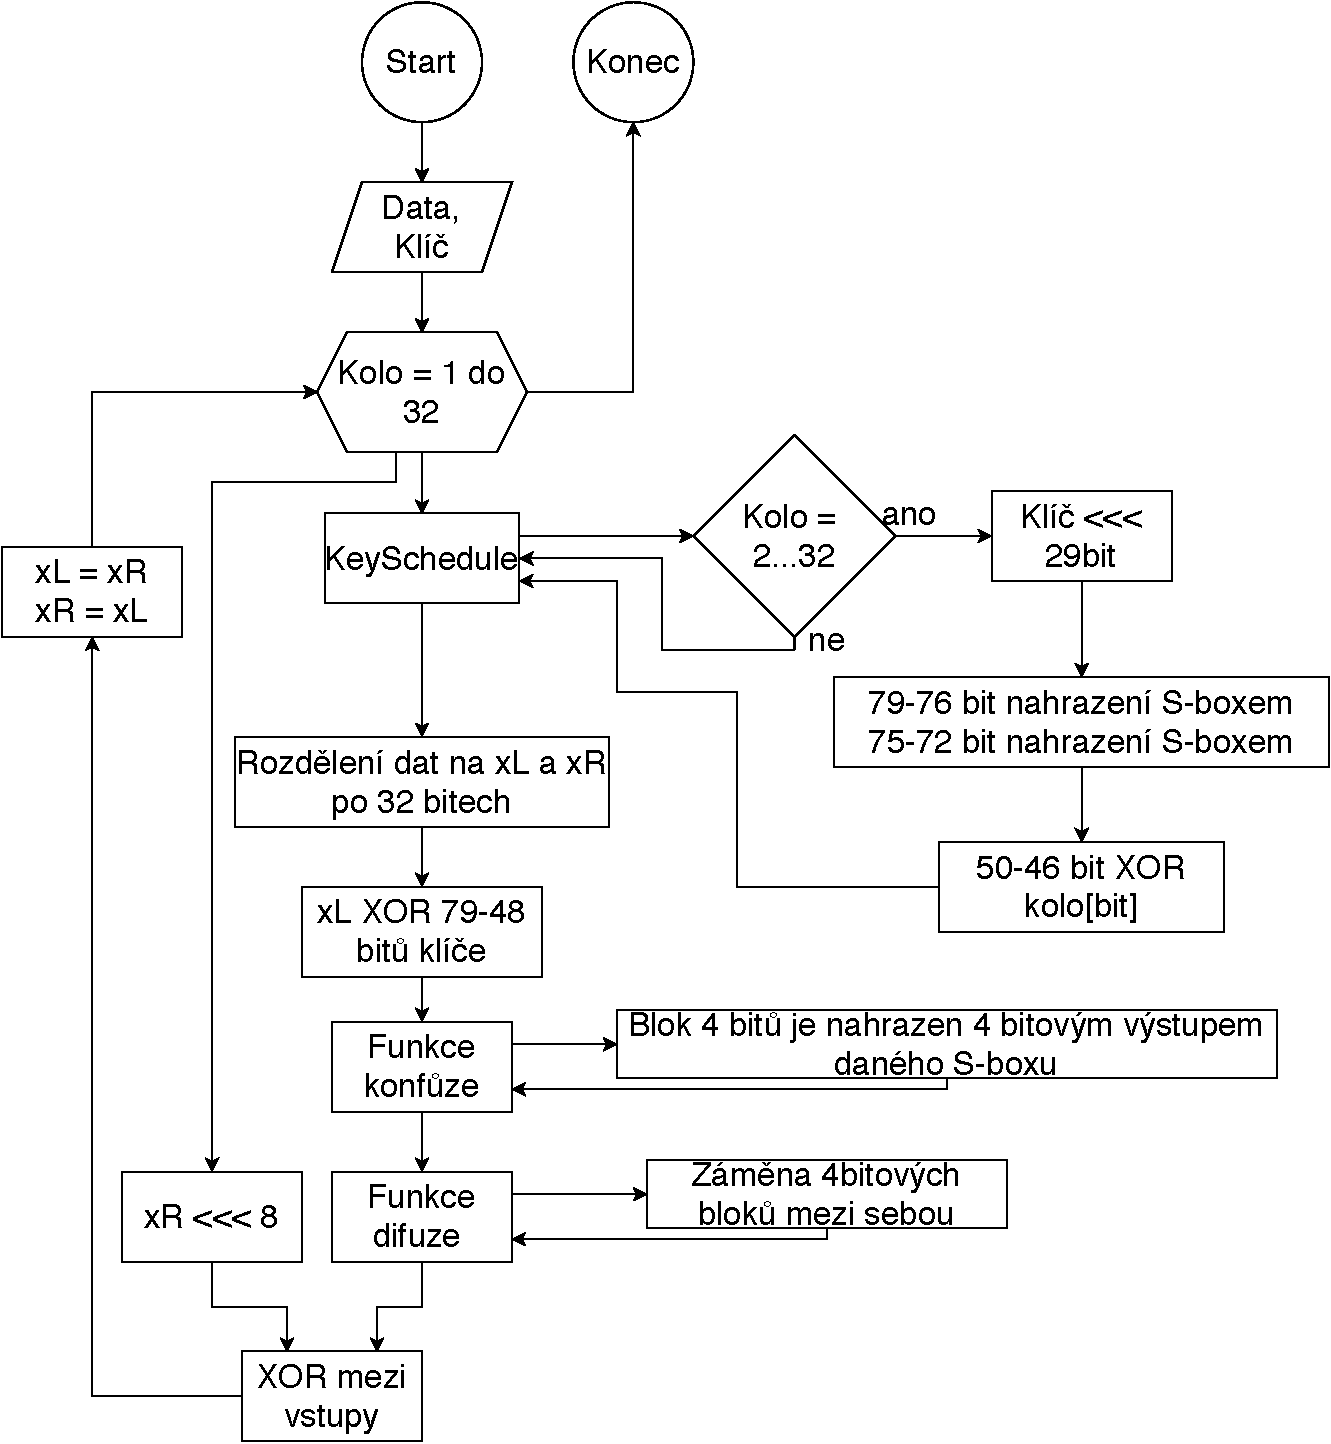
\includegraphics[scale=0.55]{obrazky/vyvojovyDiagram.pdf}
  \end{center}
  \caption[Vývojový diagram šifry LBlock]{Vývojový diagram šifry LBlock.}
  \label{img:vyvojovyDiagram}
\end{figure}

\noindent Tyto části budou podrobněji probrány v~následujících podkapitolách, pod názvy RoundFunction, ConfusionFunction, DiffusionFunction, KeySchedule, LBlockLoop a LBlockTop.

\subsection{Implementace KeySchedule}
Implementace tohoto procesu je založena na úpravě klíče v každém kole, kromě prvního. V~prvním kole se vezme prvních 32\,bitů z~levé strany vstupního klíče. V~následujících kolech to jsou kola 2-32. V~těchto kolech probíhají operace bitového posunu jako rotace o~29\,bitů. Tento posun je na řádku 1~ve \vypis{vyp:keySchedule}. Zde je využit vnitřní signál procesu, který slouží jako proměnná pro bitový posun klíče. Funkce S9 řádek 3 a S8 řádek 9 je využití S-boxů, které se aplikují na prvních 8\,bitů rozdělených do dvou stejně dlouhých bitových bloků. Řádky 15 až 18 definují zbylých 72\,bitů, kdy se s~bity 50-46 a bitovou hodnotou aktuálního kola provádí operace XOR.
\lstset{
numbers=left
}
\begin{lstlisting}[language=VHDL, caption=Key schedule, frame=single, label={vyp:keySchedule}]
switched <= key_in(50 downto 0) & key_in(79 downto 51);

    S9 : Sbox9 
        port map (
            data_in => switched(79 downto 76),
            data_out => key_out(79 downto 76)
    );
    
    S8 : Sbox8
        port map (
            data_in => switched(75 downto 72),
            data_out => key_out(75 downto 72)   
    );
    
    key_out(71 downto 51) <= switched(71 downto 51);
    key_out(50 downto 46) <= switched(50 downto 46) 
    XOR round_value(4 downto 0);
    key_out(45 downto 0) <= switched(45 downto 0);
\end{lstlisting}
\subsection{Implementace ConfusionFunction\label{subsec:confusion}}
Implementace modulu ConfusionFunction funguje na principu tzv. obalu neboli modul volá několik submodulů. Vstupem uvedeného modulu je blok o~velikosti 32\,bitů. Tento modul následně volá 8~submodulů, které implementují dané S-boxy $s_7$\,--\,$s_0$. Vstupem každého S-boxu je 4bitový blok, kde do S-boxu $s_7$ jdou první 4 nejvýznamnější bity a~následně se k dalším S-boxům přiřazují 4bitové bloky sestupně od nejvýznamnějšího bloku. Výstupem těchto submodulů jsou přeměněné bloky bitů, které se následně spojují do výstupního 32bitového bloku v~pořadí $s_7$\,--\,$s_0$. Tento 32bitový blok je výsledným výstupem modulu ConfusionFunction.

\subsection{Implementace DiffusionFunction\label{subsec:diffusion}}
Modul DiffusionFunction je jednoduchou implementací funkce difuze. Funguje na principu vstupu 32bitového bloku dat. Blok je rozdělen na menší 4bitové bloky, které se následně vyměňují mezi sebou. Tato výměna se vždy opakuje po čtyřech 4bitových blocích. Výměna probíhá následovně tak, že první blok se přemísťuje na třetí pozici, druhý blok se přemísťuje na první pozici, třetí blok na čtvrtou pozici a~čtvrtý blok na druhou pozici. Popsaný proces výměny proběhne dvakrát tzn. že pro každou polovinu vstupního bloku daný postup bude vykonán jednou. Po procesu výměny se všechny tyto 4bitové bloky spojí do 32bitového výstupního bloku, který je zároveň výstupem uvedeného modulu. Na \obrazek{img:diffusionBlock} je znázorněn postup výměny čtyř 4bitových bloků.
\begin{figure}[!h]
  \begin{center}
    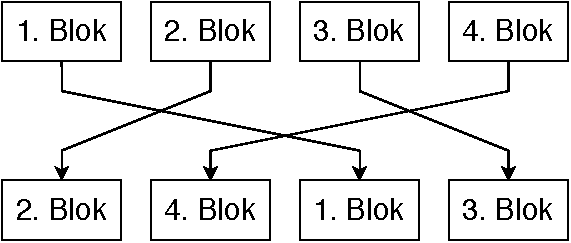
\includegraphics[scale=0.6]{obrazky/diffusionBlock.pdf}
  \end{center}
  \caption[Výměna čtyř 4bitových bloků]{Výměna čtyř 4bitových bloků.}
  \label{img:diffusionBlock}
\end{figure}

\subsection{Implementace RoundFunction\label{subsec:round}}
Modul RoundFunction se stará o~imlementaci funkce kola \textit{F}. Vstupem do modulu je aktuální klíč kola a~blok dat z~levé strany Fiestelovy sítě. V počáteční části se zavolá submodul, který má za úkol vyextrahovat ze vstupního 80bitového klíče prvních 32\,bitů. Tento submodul je vytvořen hlavně z~důvodu přehlednosti a~čitelnosti kódu. Vyextrahovaný klíč se uloží do interního signálu, nesoucí název key32bit. Následně je vypočítán interní signál resultOfXOR, který je výsledkem operace XOR mezi key32bit a~vstupním blokem dat. Volá se submodul Sbox popsaný v~\fullref{subsec:confusion}. Jeho vstupem je signál resulOfXOR a~výstupem interní signál resultOfSbox. V~poslední části se volá modul popsaný v~\fullref{subsec:diffusion}, který využívá signál resultOFSbox jako vstupní blok dat. Výstupní data modulu, který implementuje funkci difuze, jsou uložena do výstupu modulu RoundFunction.

\subsection{Implementace LBlockLoop\label{subsec:loop}}
V~tomto modulu se uskutečňuje celé kolo pro šifru LBlock. Vstupem je 80bitový klíč, levá a~pravá strana Fiestelovy sítě. Výstupem je pravá strana, která je rovna hodnotě na vstupu levé strany a~levá strana, která je výstupem úprav kola. Tyto úpravy se uvádí v postupných krocích. Nejprve se zavolá modul RoundFunction, který byl popsán v~\fullref{subsec:round}. Data pravé vstupní strany, která se upraví bitovou rotací o~8\,bitů, se uloží do interního signálu shifted. Na tento signál společně s~výstupem RoundFunction je následně použita operace XOR. Výsledek exkluzivní disjunkce je použit na výstup levé strany. Celý postup ve VHDL je znázorněn na \vypis{vyp:loop}.
\begin{lstlisting}[language=VHDL, caption=LBlockLoop, frame=single, label={vyp:loop}]
RF : RoundFunction 
    port map (
        key_in => fullKey_in,
        xL_in => xLdata_in,
        xL_out => xLhelp
    );

shifted <= xRdata_in(23 downto 0) & 
           xRdata_in(31 downto 24);

dataHelp <= shifted XOR xLhelp;

xLdata_out <= dataHelp;
xRdata_out <= xLdata_in;
\end{lstlisting}

\subsection{Implementace LBlockTop}
V~modulech obsahující slovo \uv{top} bývá nejčastěji uložena ovládací logika ostatních modulů. Moduly s tímto přívlastkem se používají k~lepší organizaci hierarchie souborů. Tento modul implementuje časování každého kola pomocí signálu cls (clock). Při nástupu hrany cls neboli změny hodnoty z~0 na 1, se provede jedno celé kolo šifry LBlock a~úpravy klíče. Signál nxState se skládá ze tří stavů, tyto stavy jsou WAITDATA, ROUND a~FINAL. Když je signál ve stavu WAITDATA, načítá se hodnota klíče a~data do interních signálů. Dále se nastaví hodnota kola a~nový stav ROUND. Při stavu ROUND se nastavují hodnoty signálů z~volaných modulů KeySchedule a~LblockLoop, aby mohly být použity jako vstupní signály při další nástupní hraně clk. Dále se zde inkrementuje hodnota kola a~kontroluje se zda hodnota kola nedosáhla 32. Jestliže hodnota je rovna 32, data se zapíší na výstup a~hodnota stavu se změní na FINAL. Nastane-li hodnota menší než 32, stav se nezmění a~klíč pro další kolo bude předán signálu klíče.

\begin{lstlisting}[language=VHDL, caption=LBlockTop, frame=single, label={vyp:loop}]
process(clk, reset)
begin
    elsif CLK'EVENT and clk = '1' then
        case nxState is
            when WAITDATA =>
                RoundFullKey <= Key_in;
                xLdata_in_intern <= data_in(63 downto 32);
                xRdata_in_intern <= data_in(31 downto 0);
                busy <= '1';
                nxState <= ROUND;
                roundCounter <= "000001";
                    
            when ROUND =>
                xLdata_in_intern <= xLdata_out_intern;
                xRdata_in_intern <= xRdata_out_intern;
                roundCounter <= roundCounter + '1';
               if roundCounter = "100000" then
                    data_out <= xRdata_out_intern &
                                xLdata_out_intern;
                    nxState <= FINAL;
                else
                    nxState <= ROUND;
                    roundFullKey <= roundKeyHelp;
                end if;
        end case;
    end if;
end process;
\end{lstlisting}
\section{Testovaní správné implementace šifry}
Testovaní je založeno na kontrole výstupních dat pomocí simulace ve 
Vivado Design Suite. Existují dvě metody zadávání vstupů do simulace. Těmito metodami je zadávání vstupů automatizovaně nebo manuálně.

Manuální zadávání vstupních signálů je vhodné, jestliže máme malý vzorek vstupů a neprovádíme tyto testy opakovaně. V dlouhodobém časovém úseku jsou tyto testy považovány za příliš komplikované, jelikož při každém testu musíme nastavit dané hodnoty manuálně.

Automatizované testy se využívají ke kontrole více hodnot a jakmile jsou napsány, lze je opakovaně simulovat. Testy se implementují pomocí tzv. testovacího stolu (anglicky testbench). Výsledky těchto testů mohou být kontrolovány manuálně nebo automatizovaně. V~práci jsou použity pouze testy s~manuální kontrolou. Výsledky simulace jsou manuálně kontrolovány s~dodanými tabulkami v~dokumentaci šifry (\emph{Wenling, 2011}\cite{LBlock}) nebo vlastnoručně vypočtenými hodnotami. 

Za nejdůležitější lze považovat testovaní implementace celé šifry, která se nachází v~modulu LBlockTop. Zde byly aplikovány dvě testovací hodnoty vytvořené tvůrci šifry LBlock, které byli využity pro testovaní. Jedná se dva vstupní bloky a~dva klíče, jak je patrné z~\tabulky{tab:testLBlock}.

\begin{table}[!h]
\addtolength{\parindent}{-5mm}
\centering
\caption[Výsledné vektory pro LBlock]{\label{tab:testLBlock}Výsledné vektory pro LBlock v hexadecimalním tvaru\,\cite{LBlock}.}
\begin{tabular}{| >{\centering\arraybackslash}p{3mm}| >{\centering\arraybackslash}p{3.85cm} | >{\centering\arraybackslash}p{5cm} | >{\centering\arraybackslash}p{3.85cm} |}
\hline
 & Zpráva & Klíč & Šifrovaný text\\ \hline
 1 & 00\,00\,00\,00\,00\,00\,00\,00 & 00\,00\,00\,00\,00\,00\,00\,00\,00\,00 & c2\,18\,18\,53\,08\,e7\,5b\,cd\\ \hline
 2 & 01\,23\,45\,67\,89\,ab\,cd\,ef & 01\,23\,45\,67\,89\,ab\,cd\,ef\,fe\,dc & 4b\,71\,79\,d8\,eb\,ee\,0c\,26 \\ \hline
 \end{tabular}
\end{table}

Hodnoty zprávy a~klíče z~\tabulky{tab:testLBlock} byli použity jako vstupy, kdy výsledný šifrovaný text odpovídal hodnotám dosažených v~testové simulaci. Oba dva výsledky lze vidět na \obrazek{img:test0} pro zprávu 1, respektive na \obrazek{img:test1} pro zprávu 2.

\begin{figure}[!h]
  \begin{center}
    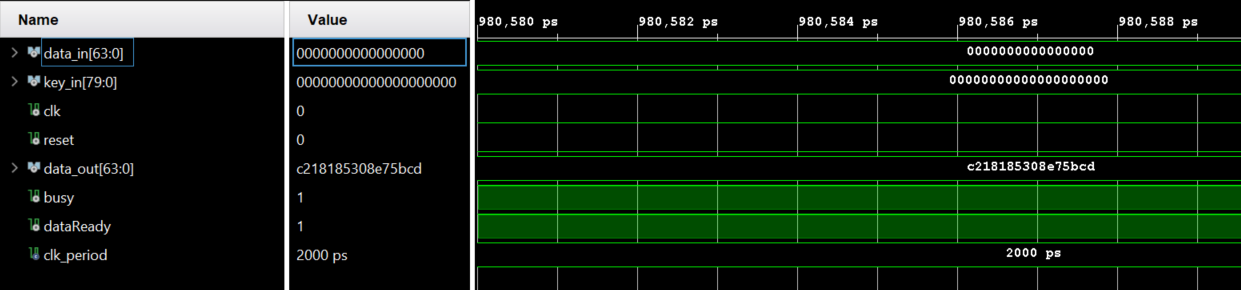
\includegraphics[scale=0.57]{obrazky/test0.PNG}
  \end{center}
  \caption[Výsledek simulace pro zprávu 1]{Výsledek simulace pro zprávu 1.}
  \label{img:test0}
\end{figure}
\newpage
\begin{figure}[t]
  \begin{center}
    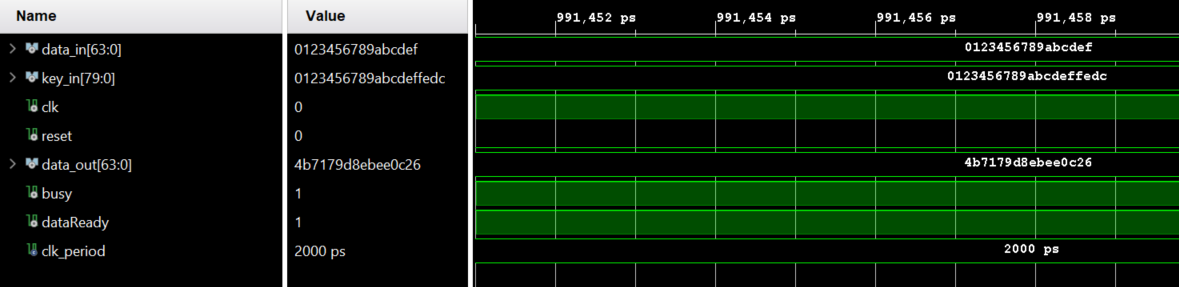
\includegraphics[scale=0.57]{obrazky/test1.PNG}
  \end{center}
  \caption[Výsledek simulace pro zprávu 2]{Výsledek simulace pro zprávu 2.}
  \label{img:test1}
\end{figure}
\null
\vfill